\documentclass[12pt, french]{article}

\usepackage{fancyhdr, fancybox, lastpage}
\usepackage[most]{tcolorbox}
\usepackage[a4paper, margin={0.3in, .75in}]{geometry}
\usepackage{wrapfig}
\pagestyle{fancy}
\renewcommand\headrulewidth{1pt}
\renewcommand\footrulewidth{1pt}
\fancyhf{}
\rhead{ \em{Zakaria Haouzan}}
\lhead[C]{\em{1ére année baccalauréat Sciences Expérimentales}}
\chead[C]{}
\rfoot[C]{}
\lfoot[R]{}
\cfoot[]{\em{Page \thepage / \pageref{LastPage}}}


\newtcolorbox{Box2}[2][]{
                lower separated=false,
                colback=white,
colframe=white!20!black,fonttitle=\bfseries,
colbacktitle=white!30!gray,
coltitle=black,
enhanced,
attach boxed title to top left={yshift=-0.1in,xshift=0.15in},
title=#2,#1}


\begin{document}
\begin{center}
   \shadowbox {\bf{ ÉNERGIE POTENTIELLE DE PESANTEUR - ÉNERGIE MÉCANIQUE }}
\end{center}


%%_________________________Exercice !2 :"_________________________Exercice
\begin{Box2}{Exercice 1 : }
Sara, debout sur un pont, lance verticalement vers le haut une pierre de masse
m = 70 kg.
La pierre s’élève jusqu’à une hauteur de 10 m au-dessus du pont de lancement puis
redescend et tombe dans l’eau.
La surface de l’eau est située 2 m plus bas que le point de lancement de la pierre.

  1. calculer :

  L’énergie potentielle de pesanteur de la pierre dans sa position la plus haute.

  L’énergie potentielle de pesanteur de la pierre dans sa position la plus basse.
 
  La variation de l’énergie potentielle de pesanteur de la pierre.

  Si l’on choisit comme niveau de référence (origine de l’axe Oz dirigé vers le haut)
 
  1.1. Le niveau du point de lancement de la pierre.
 
  1.2. Le niveau de la surface de l’eau.

  2. Quel conclusion pouvez-vous en tirer ?
\end{Box2}

%%_________________________Exercice ! :"_________________________Exercice
   \begin{Box2}{Exercice 2 : }
      Une balle de masse m = 200 g est lancé verticalement vers le haut avec une vitesse de valeur $5,0 m.s^{-1}$ à partir d'un point situé à 1,20 m du sol.

1. Calculer les énergies potentielle, cinétique et mécanique de la balle à l'état initial.

2. Calculer l'altitude maximale de la balle lors de ce lancer.

3. Calculer la vitesse de la balle au moment où elle retombe sur le sol.
      Donnée : $g = 9,8 N.kg^{-1}$ .
   \end{Box2}


%%_________________________Exercice ! 3:"_________________________Exercice
\begin{Box2}{Exercice 3 :}
Une pomme de masse m = 150g, accrochée à un pommier, se trouve à 3,0 m audessus du sol. Le sol est choisi comme référence des énergies potentielles de
pesanteur.
On donne g = 10 N/Kg

1. Lorsque cette pomme est accrochée au pommier, quelle est :
 
  a. son énergie cinétique ?
 
  b. son énergie potentielle de pesanteur ?
 
  c. son énergie mécanique ?

  2. la pomme se détache et arrive au sol avec une vitesse de valeur V= 7,75 m/s.

  Calculer :
 
  a. son énergie cinétique.

  b. son énergie potentielle de pesanteur.
 
  c. son énergie mécanique.

  3. Quelles transformations énergétiques ont eu lieu au cours de cette chute ?

  4. Quelle serait la hauteur de chute de cette pomme si elle arrivait au sol avec une
vitesse de valeur V' =9,9 m/s

\end{Box2}

%%_________________________Exercice 4 : _________________________Exercice
\begin{Box2}{Exercice 4 : }
\begin{wrapfigure}{r}{0.39\textwidth}
  \begin{center}
    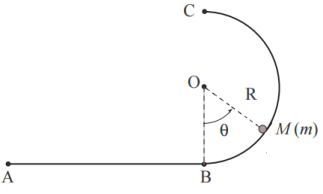
\includegraphics[width=0.37\textwidth]{./img/img03.png}
  \end{center}
\end{wrapfigure}
Un solide ponctuel de masse m est lancé en A sur une piste horizontale prolongée par un demi-cercle vertical de rayon R.
On donne : AB = 1 m ; R = 1 m ; m = 0, 5 kg ; g = 9, 81 N/kg

   1. Les frottements étant négligeables, calculer en A la vitesse minimale $V_{A_{min}}$ que doit avoir la masse pour qu’elle atteigne le point C

   2. Même question lorsque les frottements entre l’objet et la piste sont assimilables à une force constante de norme f=1N.

\end{Box2}

\vspace{2cm}
\begin{center}
   \Large{ \em{Exercices Supplémentaires}}
\end{center}



%%_________________________Exercice 5 : _________________________Exercice
\begin{Box2}{Exercice 5 : }
\begin{wrapfigure}{r}{0.39\textwidth}
  \begin{center}
    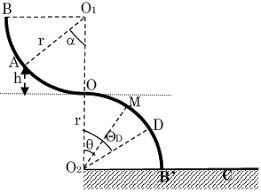
\includegraphics[width=0.37\textwidth]{./img/img04.png}
  \end{center}
\end{wrapfigure}
Une portion de gouttière BO de forme circulaire de rayon $r=1m$ se situe dans un plan
vertical. Elle se raccorde en O à une autre gouttière identique OB’ située dans le même plan (voir figure).

Les centres O1 et O2 des deux gouttières se trouvent sur la même verticale. Un solide ponctuel S de masse m=100g est lâché sans vitesse du point A situé à une hauteur h = 0,2 m par rapport au plan horizontal passant par O. Les frottements étant supposés négligeables et $g = 10kg/N$

1. En choisissant le point O comme origine des altitudes et comme position de référence, calculer l’énergie mécanique du solide.

2. Exprimer puis calculer la vitesse du solide VO au passage en O.

3. Sur le parcours OD le solide reste en contact avec la surface de la gouttière et sa position est repéré par l’angle $\theta = (\overrightarrow{O_2O}, \overrightarrow{O_2M})$
Etablir l’expression de la vitesse V du solide en un point M quelconque du trajet OD en fonction de h , r , g et $\theta$.

   4. Sur le trajet OD on montre que l’intensité R de la réaction de la gouttière sur S à pour expression $$R = mg(cos(\theta) - \frac{V^2}{r.g})$$
Au point D le solide S perd le contact avec la gouttière et suit le trajet DC. Déterminer la valeur numérique $\theta_D$ et celle de $V_D$ vitesse du S au point D.

   5. Avec quelle vitesse du solide touche-t-il le sol en C ?
\end{Box2}

\begin{Box2}{Exerice 6 : }
Un cycliste descend une pente de 10\% . Sa vitesse v = 54km/h est constante .

1. Calculer la variation de l’énergie potentielle de pesanteur pendant $\Delta$t = 1s .

2. Calculer la quantité de chaleur Q dissipée par les frottement au niveau des freins pendant 30s.

Donnée : L’ensemble cycliste -bicyclette a une masse m = 80kg L’intensité de pesanteur g = 9, 8N/kg

\end{Box2}

\begin{Box2}{Exerice 7 }
\begin{wrapfigure}{r}{0.39\textwidth}
  \begin{center}
    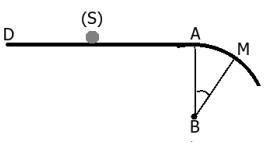
\includegraphics[width=0.37\textwidth]{./img/img05.png}
  \end{center}
\end{wrapfigure}

   Un skieur glisse sur une piste horizontale $DA$ à vitesse constante . En A, commence une portion de piste circulaire de rayon R =BA (B est à la verticale de de A ) . Les frottement sont négligeables et on admet que le skieur est assimilable à un point matériel dont la trajectoire suit la forme de la piste.

1. Calculer la variation de l’énergie mécanique enter le point A et le point M .

   2. Déduire l’expression de la vitesse de skieur au point M en fonction de R , $\theta=\Hat{ABM}$ et g
On prend g = 10N/kg

\end{Box2}
%%_________________________Exercice 6 : _________________________Exercice
\end{document}
